\documentclass[11pt,a4paper,oneside,english]{amsart}

\usepackage{amsaddr}
\usepackage{babel}
\usepackage{amssymb}
\usepackage{bm}
\usepackage{booktabs}
\usepackage{commath}
\usepackage{colortbl}
\usepackage{dsfont}
\usepackage{enumerate}
\usepackage{esint}
\usepackage[left=0.09\paperwidth, right=0.15\paperwidth, bottom=0.12\paperheight]{geometry}
\usepackage{graphicx}
\usepackage[displaymath, mathlines]{lineno}
\usepackage{mathtools}
\usepackage{mathrsfs}
\usepackage{multirow,bigdelim}
\usepackage{url}
\usepackage{pdflscape}
\usepackage{rotating}
%\usepackage[outer]{showlabels}
\usepackage[color=white,linecolor=black, textwidth=0.12\paperwidth]{todonotes}
%\setlength{\parindent}{0pt}
\usepackage{wrapfig}

\numberwithin{equation}{section}
\newtheorem{theorem}{Theorem}
\numberwithin{theorem}{section}
\newtheorem{assum}[theorem]{Assumption}
\newtheorem{lemma}[theorem]{Lemma}
\newtheorem{corol}[theorem]{Corollary}
\newtheorem{prop}[theorem]{Proposition}
\theoremstyle{definition}
\newtheorem{remark}[theorem]{Remark}
\newtheorem{example}[theorem]{Example}

\usepackage{color}
\newcommand{\R}{\mathbb{R}}
\newcommand{\N}{\mathbb{N}}
\newcommand{\Z}{\mathbb{Z}}
\providecommand\C{}
\renewcommand{\C}{\mathbb{C}}
\newcommand{\A}{\mathcal{A}}
\newcommand{\Q}{\mathbb{Q}}
\newcommand{\E}{\mathcal{E}}
\newcommand{\F}{\mathbb{F}}
\newcommand{\D}{\mathcal{D}}
\newcommand{\K}{\mathcal{K}}
\renewcommand{\H}{\mathcal{H}}
\newcommand{\B}{\mathcal{B}}
\newcommand{\M}{\mathcal{M}}
\newcommand{\bbD}{\mathbb{D}}
\newcommand{\f}{\varphi}
\newcommand{\e}{\varepsilon}
\newcommand{\eps}{\varepsilon}
\renewcommand{\a}{\alpha}
\renewcommand{\b}{\beta}
\newcommand{\z}{\zeta}
\renewcommand{\O}{\Omega}
\renewcommand{\P}{\mathbb P}
\newcommand{\intRn}{\int_{\R^n}}
\newcommand{\sumi}{\sum_{i=1}^n}
\newcommand{\sumij}{\sum_{i,j=1}^n}
\renewcommand{\d}{\delta}
\newcommand{\p}{\partial}
\DeclareMathOperator{\osc}{osc}
\DeclareMathOperator{\supp}{supp}
\DeclareMathOperator{\vol}{vol}
\DeclareMathOperator{\gen}{gen}
\DeclareMathOperator{\cat}{Cat}
\DeclareMathOperator{\Cat}{Cat}
\DeclareMathOperator{\Div}{div}
\DeclareMathOperator{\blockdiag}{blockdiag}
\renewcommand{\div}{\Div}
\providecommand{\spann}{\mathrm{span}}
\providecommand{\diam}{\mathrm{diam}}
\providecommand{\dist}{\mathrm{dist}}
\newcommand{\la}{\langle}
\newcommand{\ra}{\rangle}
\usepackage{stmaryrd}
\newcommand{\jump}[1]{\left\llbracket #1 \right\rrbracket}
\newcommand{\rhu}{\rightharpoonup}
\newcommand{\T}{\mathcal{T}}
\newcommand{\V}{\mathcal{V}}
\DeclareMathOperator*{\dof}{\#\!DoF}
\DeclareMathOperator*{\argmin}{arg\,min}
\DeclareMathOperator*{\Id}{Id}
\definecolor{airforceblue}{rgb}{0.36, 0.54, 0.66}
\definecolor{ao(english)}{rgb}{0.0, 0.5, 0.0}
\providecommand\note{}
\newcommand{\new}[1]{{\color{ao(english)} #1}}
\renewcommand{\L}{\mathcal L}
\newcommand{\Y}{\mathcal Y}
\newcommand{\Lto}{{L_2(\Omega)}}
\newcommand{\bbT}{\mathbb{T}}
\newcommand{\cL}{\mathcal L}
\newcommand{\Lis}{\cL\mathrm{is}}
\newcommand{\udelta}{{\underline{\delta}}}
\newcommand{\jw}[1]{{\color{red}{JW: #1}}}
\newcommand{\rvv}[1]{{\color{teal}{RvV: #1}}}
\DeclareMathOperator*{\ran}{ran}

% Math symbol font matha
\DeclareFontFamily{U}{matha}{\hyphenchar\font45}
\DeclareFontShape{U}{matha}{m}{n}{
      <5> <6> <7> <8> <9> <10> gen * matha
      <10.95> matha10 <12> <14.4> <17.28> <20.74> <24.88> matha12
      }{}
\DeclareSymbolFont{matha}{U}{matha}{m}{n}
\DeclareFontSubstitution{U}{matha}{m}{n}

% Math symbol font mathb
\DeclareFontFamily{U}{mathx}{\hyphenchar\font45}
\DeclareFontShape{U}{mathx}{m}{n}{
      <5> <6> <7> <8> <9> <10>
      <10.95> <12> <14.4> <17.28> <20.74> <24.88>
      mathx10
      }{}
\DeclareSymbolFont{mathx}{U}{mathx}{m}{n}
\DeclareFontSubstitution{U}{mathx}{m}{n}

% Symbol definition
\DeclareMathDelimiter{\vvvert}{0}{matha}{"7E}{mathx}{"17}

\DeclareMathOperator{\ext}{ext}
\DeclareMathOperator{\eff}{eff}
\DeclareMathOperator{\loc}{loc}
\DeclareMathOperator{\irr}{int}
\DeclareMathOperator{\RT}{RT}
\DeclareMathOperator{\meas}{meas}
\newcommand{\bbone}{\mathds{1}}
\newcommand{\bbzero}{\mathds{0}}
\newcommand{\seminorm}[1]{\vvvert #1 \vvvert}
\newcommand{\ltwonorm}[1]{\lVert #1 \rVert}
\newcommand{\hta}{{\check \T_a}}
\newcommand{\hT}{{\check T}}
\newcommand{\he}{{\check e}}
\newcommand{\hE}{{\check \E}}
\newcommand{\dr}{{\tilde r}}
\renewcommand{\emptyset}{{\varnothing}}
\newcommand{\hprime}[1]{H^1_{*, #1}(\hta)}
\newcommand{\laplace}{\mathcal{4}}

\DeclareFontFamily{U}{mathx}{\hyphenchar\font45}
\DeclareFontShape{U}{mathx}{m}{n}{
      <5> <6> <7> <8> <9> <10>
      <10.95> <12> <14.4> <17.28> <20.74> <24.88>
      mathx10
      }{}
\DeclareSymbolFont{mathx}{U}{mathx}{m}{n}
\DeclareFontSubstitution{U}{mathx}{m}{n}
\DeclareMathAccent{\widecheck}{0}{mathx}{"71}
\DeclareMathAccent{\wideparen}{0}{mathx}{"75}
%\linenumbers

\def\cs#1{\texttt{\char`\\#1}}

\title{Space-time adaptivity for parabolic evolution equations}
\author{Rob Stevenson \and Raymond van Veneti\"e \and Jan Westerdiep}
\address{Korteweg-de Vries Institute for Mathematics, University of Amsterdam, \\
P.O. Box 94248, 1090 GE Amsterdam, The Netherlands}
\date{\today}
\subjclass[2010]{}

\thanks{\emph{Funding:} The second and third authors are supported by the Netherlands Organisation for Scientific Research (NWO) under contract.~no.~613.001.652}

\begin{document}
\begin{abstract}
\end{abstract}

\maketitle

\section{Introduction}
\section{Problem statement and solution}
Let $V$ and $H$ be separable Hilbert spaces on a spatial domain $\Omega$ such that
$V \hookrightarrow H$ with dense and compact embedding. Identifying $H$ with its
dual, we obtain the Gelfand triple $V \hookrightarrow H \simeq H' \hookrightarrow V'$.

We use the notation $\la \cdot,\cdot \ra$ to denote both the scalar product
on $H \times H$, and its unique extension by continuity to the duality pairing on
$V' \times V$. Correspondingly, the norm on $H$ will be denoted by $\|\cdot\|$.

Let $T \in (0, \infty)$ be given, and set $I := (0, T)$. We make the following assumption.
\begin{assum}
  \label{assum:a}
  For a.e. $t$, let $a(t;\cdot,\cdot)$ denote a bilinear form on $V \times V$ that is
  \begin{alignat*}{3}
    t \mapsto a(t; \eta, \zeta) & ~~ \text{is measurable} \quad && (\eta, \zeta \in V) \\
    |a(t;\eta,\zeta)| & \lesssim  \|\eta\|_{V} \|\zeta\|_{V} &&(\eta,\zeta \in V) &&\text{(bounded)}, \\
     a(t;\eta,\eta)   & \gtrsim   \|\eta\|_{V}^2 &&(\eta \in {V}) &&\text{(coercive)}.
  \end{alignat*}
\end{assum}

With $A(t) \in \Lis({V},V')$ being defined by $ (A(t) \eta)(\zeta)=a(t;\eta,\zeta)$,
we are interested in solving the {\em parabolic initial value problem} of finding
$u$ such that
\begin{equation}
  \label{eqn:ibvp}
  \left\{
    \begin{array}{rl} 
      \frac{\dif u}{\dif t}(t) +A(t) u(t)&\!\!\!= g(t) \quad(t \in I),\\
      u(0) &\!\!\!= u_0.
    \end{array}
  \right.
\end{equation}

In a simultaneous space-time variational formulation, the parabolic PDE reads as
finding $u$ from a suitable space of functions of time and space such that
\begin{equation}
  \label{eqn:B-var-form}
  (Bw)(v):=\int_I \la \tfrac{\dif w}{\dif t}(t), v(t) \ra + a(t;w(t),v(t)) \dif t = \int_I \la g(t), v(t) \ra =:g(v)
\end{equation}
for all $v$ from another suitable space of functions of time and space.

\begin{theorem}
  \label{thm:varform}
  With $X:=L_2(I;{V}) \cap H^1(I;V')$, $Y:=L_2(I;{V})$, under assumption \ref{assum:a}, we have
  \begin{equation}
    \label{eqn:B-lis}
    \begin{bmatrix} B \\ \gamma_0\end{bmatrix}\in \Lis(X,Y' \times H),
  \end{equation}
  where for $t \in \bar I$, $\gamma_t\colon u \mapsto u(t,\cdot)$ denotes the trace map.
  In other words, given $(g, u_0) \in Y' \times H$, finding $u \in X$ such that 
  \begin{equation}
    \label{eqn:B-varform}
    (Bu)(v_1)+\la u(0,\cdot),v_2\ra=g(v_1)+\la u_0,v_2\ra\quad ((v_1,v_2) \in Y \times H),
  \end{equation}
  is a well-posed variational formulation of \eqref{eqn:ibvp}.
\end{theorem}

\subsection{Andreev formulation}
Defining $A, A_s \in \Lis(Y,Y')$, $A_a \in \cL(Y,Y')$, and $\partial_t \in \cL(X,Y')$ by 
\[
(Au)(v):=\int_I a(t;u(t),v(t)) \dif t, \quad A_s:=\tfrac12(A+A'), \quad A_a:=\tfrac12(A-A'), \quad \partial_t:=B-A,
\]
an equivalent self-adjoint saddle point formulation of \eqref{eqn:B-varform} was
introduced by Andreev in \cite{Andreev2013} as finding the solution $(\mu,u) \in Y\times X$ of
\[
  \begin{bmatrix} A_s & B\\ B' & -\gamma_0' \gamma_0 \end{bmatrix}
  \begin{bmatrix} \mu \\ u \end{bmatrix}=
  \begin{bmatrix} g \\ -\gamma_0' u_0 \end{bmatrix}.
\]
Thanks to \eqref{eqn:B-lis}, the Schur complement $S := B' A_s^{-1} B+\gamma_0'\gamma_0$ is in $\Lis(X, X')$, is self-adjoint, and coercive.

\begin{remark}
  For some quantitative estimates to be valid, we assume that $A=A_s$, but we do not expect this to be essential.
\end{remark}
We equip $Y$ and $X$ with the `energy' norms
$$
\|\cdot\|_Y^2:=(A_s\cdot)(\cdot),\quad \|\cdot\|_X^2:=\|\cdot\|_Y^2+\|\partial_t \cdot\|_{Y'}^2+\|\gamma_T \cdot\|^2,
$$
which are equivalent to the canonical norms on $Y$ and $X$.

\begin{lemma}
  \label{lem:energy-norm}
  It holds that $\|\cdot\|_X^2=(S\cdot)(\cdot)$.
\end{lemma}
\begin{proof} 
  We find \jw{dit ben ik nog niet nagegaan}
  \[
    \|w\|_X^2=\sup_{0 \neq v_1 \in Y} \frac{(B w)(v_1)}{\|v_1\|_Y^2}+\|\gamma_0 w\|^2
    =\sup_{0 \neq (v_1,v_2) \in Y \times H} \frac{((B w)(v_1)+\la \gamma_0 w,v_2\ra)^2}{\|v_1\|_Y^2+\|v_2\|^2} =(Sw)(w),
  \]
  where the first equality can be found in e.g.~\cite[Thm.~2.1]{Ern2017a}, and,
  when realising that $S$ is also the Schur complement of 
  $\begin{bsmallmatrix} A_s & 0 & B\\ 0 & \Id & \gamma_0\\ B' & \gamma_0' & 0\end{bsmallmatrix} \in \cL(Y\times H \times X, Y'\times H'\times X')$, the last one follows from e.g.~\cite[Lemma~2.2]{Kondratyuk2008}.
\end{proof}

Let $(X^\delta)_{\delta \in \Delta}$ be a collection of closed subspaces of $X$. 
We define a \emph{partial order} on $\Delta$ by $\delta \preceq \tilde{\delta}$
when $X^\delta \subseteq X^{\tilde{\delta}}$. For $\delta \in \Delta$, let
$u_\delta \in X^\delta$ denote the {\em Galerkin approximation to $u$}, i.e., the solution of
\begin{equation}
(Su_\delta)(v)=f(v) \quad (v \in X^\delta), 
  \label{eqn:galerkin}
\end{equation}
being the best approximation to $u$ from $X^\delta$ w.r.t.~$\|\cdot\|_X$.

\subsection{Discretized problem}
Applying $S$ requires the application of the nonlocal operator $A_s^{-1}$, making it
unsuitable for practical computation. To that end, let $(Y^\delta)_{\delta \in \Delta}$
be a collection of closed subspaces of $Y$ satisfying $X^\delta \subseteq Y^\delta$
that is \emph{uniformly inf-sup stable}, i.e.
\begin{equation}
  \gamma_\Delta:=\inf_{\delta \in \Delta}\inf_{0 \neq w \in X^\delta}\sup_{0\neq y^\delta \in Y^\delta} \frac{(\partial_t w)(v)}{\|\partial_t w\|_{Y'}\|v\|_Y} \in (0,1].
  \label{eqn:infinfsup}
\end{equation}
Uniform stability essentially establishes the norm equivalences
\[
  \gamma_\Delta ||\partial_t w||_{Y'} \leq ||\partial_t w||_{{Y^\delta}'} \leq ||\partial_t w||_{Y'} \quad (w \in Y, \delta \in \Delta).
\]
Note that $\gamma_\Delta$ can be made arbitrarily close to $1$ by selecting $Y^\delta$ sufficiently large.

For $\delta, \hat{\delta} \in \Delta$ with $Y^{\hat{\delta}} \supseteq Y^\delta$, and 
$E_Y^{\hat{\delta}}$, $E_X^\delta$ denoting the embeddings $Y^{\hat{\delta}} \rightarrow Y$,
$X^\delta \rightarrow X$, let $(\mu^{\hat{\delta} \delta},u^{\hat{\delta} \delta}) \in Y^{\hat{\delta}} \times X^\delta$ be the solution of 
\[
  \begin{bmatrix}{E_Y^{\hat{\delta}}}' A_s E_Y^{\hat{\delta}}& {E_Y^{\hat{\delta}}}' B E^\delta_X\\ {E^\delta_X}' B' E_Y^{\hat{\delta}}& -{E^\delta_X}' \gamma_0' \gamma_0 E^\delta_X \end{bmatrix}
  \begin{bmatrix} \mu^{\hat{\delta} \delta} \\ u^{\hat{\delta} \delta} \end{bmatrix}
  \begin{bmatrix} {E^{\hat{\delta}}_Y}' g \\ -{E^\delta_X}' \gamma_0' u_0 \end{bmatrix}
\]
or
\begin{equation}
  \label{eqn:discr-schur}
  \underbrace{
    {E^\delta_X}'(B' E^{\hat{\delta}}_Y({E^{\hat{\delta}}_Y}' A_s E^{\hat{\delta}}_Y)^{-1} {E^{\hat{\delta}}_Y}' B +\gamma_0'\gamma_0)E^\delta_X
  }_{S^{\hat{\delta} \delta}:=}u^{\hat{\delta} \delta}
  =
  \underbrace{
    {E^\delta_X}' (B' E^{\hat{\delta}}_Y({E^{\hat{\delta}}_Y}' A_s E^{\hat{\delta}}_Y)^{-1} {E^{\hat{\delta}}_Y}' g+\gamma_0' u_0)
  }_{f^{\hat{\delta} \delta}:=}.
\end{equation}\rvv{heavy notatie uitstellen?}
Unless $Y^{\hat{\delta}}=Y$, it holds that $S^{\hat{\delta} \delta} \neq {E_X^\delta}' S E_X^\delta$ and $f^{\hat{\delta} \delta} \neq {E_X^\delta}'f$, and so generally $u^{\hat{\delta} \delta} \neq u_\delta$.

Equipping $X^\delta$ with `energy' norm $\|w\|^2_{X^{\hat{\delta}\delta}}:=\|w\|^2_{Y}+ \|\partial_t w\|_{{Y^\delta}'}+\|\gamma_T w\|^2$,
from \cite[Lemma~3.3]{Stevenson2020a} it follows that
$\|\cdot\|_{X^{\hat{\delta}\delta}}^2=(S^{\hat{\delta}\delta}\cdot)(\cdot)$,
similar to Lemma~\ref{lem:energy-norm}. As shown in \cite[Thm.~3.6]{Stevenson2020a}, we have
\begin{equation}
  \label{eqn:galerkin-ortho}
  \|u-u^{\hat{\delta}\delta}\|_X \leq \gamma_\Delta^{-1} \|u-u_\delta\|_X,
\end{equation}
whereas by definition of $\gamma_\Delta$ it holds that
\begin{equation}
  \label{eqn:X-norm-equiv}
  \gamma_\Delta\|\cdot\|_{X} \leq \|\cdot\|_{X^{\hat{\delta}\delta}} \leq \|\cdot\|_{X} \quad\text{on } X^\delta.
\end{equation}

\section{Realization of uniform inf-sup stability \eqref{eqn:infinfsup}}
In our previous work, we realized the inf-inf-sup condition \eqref{eqn:infinfsup}
for families $(Y^\delta, X^\delta)_{\delta \in \Delta}$ of finite element spaces
wrt.~partitions of the spacetime domain into prismatic elements, where the partition
in time is independent of the spatial location, and the spatial mesh in each
\emph{time slab} is such that the corresponding $H$-orthogonal projection is
uniformly $V$-stable.

Let us first argue why uniform stability for general nonuniform prismatic partitions
is out of reach. \jw{follows from $\dim Y^\delta \lesssim \dim X^\delta$ en
de non-locality van $A_s^{-1}$: gegeven een $X^\delta$ die naar een spacetime-hoekje
gerefined is, moet $Y^\delta$ de gehele time-slab refinen. Ik ben het precieze argument
even vergeten maar met een plaatje wordt het snel duidelijk.}

\subsection{The spatial meshes}
The following result generalizes \cite[Lemma 6.2]{11} and \cite[Proposition 2.5]{258.4}
by allowing $W \neq \tilde W$.

\begin{prop} \label{prop:space-infsup}
  Let $W$ and $\tilde W$ be closed subspaces of $H$ such that there exists a
  (biorthogonal) projector $Q \in \cL(H,H)$ with $\ran Q=W$ and $\ran (\Id -Q)={\tilde W}^\perp$. 
  Then, when $W \subset V$, it holds that 
  \[
    \gamma:=\inf_{0 \neq \tilde w \in \tilde W}\sup_{0 \neq w \in W}\frac{\la \tilde w,w\ra}{\|\tilde w\|_{V'}\|w\|_V}>0
  \]
  if and only if $Q \in \cL(V,V)$, in which case $\gamma=\|Q\|_{\cL(V,V)}^{-1}$.
\end{prop}
\begin{proof} \jw{Dit ben ik nog niet nagegaan.} If $Q\in \cL(V,V)$, then for $\tilde w \in \tilde W$,
$$
\sup_{0 \neq w \in W}\frac{\la \tilde w,w\ra}{\|w\|_V}=\sup_{0 \neq v \in V}\frac{\la \tilde w, v\ra}{\|Qv\|_V}
\geq \|Q\|_{\cL(V,V)}^{-1} \|\tilde w\|_{V'},
$$
or $\gamma \geq \|Q\|_{\cL(V,V)}^{-1}$. If on the other hand $\gamma>0$, then for any $u \in H$,
$$
\gamma \|Q' u\|_{V'} \leq \sup_{0 \neq w \in W}\frac{\la Q'u,w\ra}{\|w\|_V} =
 \sup_{0 \neq w \in W}\frac{\la u,w\ra}{\|w\|_V} \leq \|u\|_{V'},
 $$
so that from $H$ being dense in $V'$, $\|Q\|_{\cL(V,V)}=\|Q'\|_{\cL(V',V')}\leq \gamma^{-1}$.
\end{proof}
\begin{remark}
  In the typical case where $H = L_2(\Omega)$ and $V = H_0^1(\Omega)$ on a bounded
  polytopal domain $\Omega \subset \R^d$, the uniform boundedness of $\|Q\|_{\cL(V,V)}$
  has been demonstrated for families of locally refined partitions, for $d=2$
  including those that are generated by the newest vertex bisection algorithm.
  We refer to \cite{Carstensen2001a,Gaspoz2016}. \jw{Misschien is het ``$H^1$-stability
  of $L^2$-projection" inmiddels wel uitgespeeld. ik vond ook een werk uit
  2014 van de groep van Dirk, en dit werkte voor elke dimensie, maar enkel op
  vreemde fin.elts. Ook een werk uit 2019 van Gaspoz, Heine, Siebert waar het
  2d-NVB geval wordt bekeken voor Lagrange-fin elts tot graad 4.}
\end{remark}

\subsection{Wavelets in time, finite elements in space}
Let ${\mathcal O}$ be a collection of pairs of closed subspaces $(W,\tilde{W})$
as in Proposition~\ref{prop:space-infsup} with uniform inf-sup constant $\gamma>0$.

Let $\Sigma=\{\sigma_\lambda : \lambda \in \vee_\Sigma\}$ be, properly scaled, a Riesz basis for $L_2(I)$ and $H^1(I)$.\rvv{Definitie maken ergens?}
Let $\Psi=\{\psi_\lambda \colon \lambda \in \vee_\Psi\}$ be a Riesz basis for $L_2(I)$, with dual basis denoted as $\tilde{\Psi}$.

Given
\[
\framebox{$X^\delta=\sum_{\lambda \in \vee_\Sigma} \sigma_\lambda \otimes \tilde{W}_\lambda^\delta,$}
\]
where \framebox{$(W_\lambda^\delta,\tilde{W}_\lambda^\delta) \in {\mathcal O}$
or $W_\lambda^\delta=\tilde{W}_\lambda^\delta=\{0\}$}, let
\[
\framebox{$Y^\delta=\sum_{\mu \in \vee_\Psi} \psi_\mu \otimes V_\mu^\delta$}
\]
and $\tilde{Y}^\delta=\sum_{\mu \in \vee_\Psi} \tilde{\psi}_\mu \otimes \tilde{V}_\mu^\delta$ 
where \framebox{$(V^\delta_\mu,\tilde{V}^\delta_\mu) \in {\mathcal O}$ or $V_\lambda^\delta=\tilde{V}_\lambda^\delta=\{0\}$} is such that 
\begin{equation}
  \label{eqn:pre-doubletree}
  \la \sigma'_\lambda,\psi_\mu\ra_{L_2(I)} \neq 0 \implies \tilde{V}^\delta_\mu \supset \tilde{W}^\delta_\lambda.
\end{equation}
\jw{hoe werkt deze eis precies?}
Thanks to $\sigma'_\lambda=\sum_{\mu \in \vee_\Psi} \la \sigma'_\lambda,\psi_\mu\ra_{L_2(I)}\tilde{\psi}_\mu$, the previous implication ensures that
\begin{equation}
  \label{eqn:d_tX-in-Y}
 \framebox{$\partial_t X^\delta \subset \tilde{Y}^\delta.$}
\end{equation}
\rvv{deze uitlijning is slecht}
\begin{theorem}
In the previous notation, $(X^\delta,Y^\delta)_{\delta \in \Delta}$ satisfies
  \eqref{eqn:infinfsup} with uniform inf-sup constant $\gamma$.
\end{theorem}
\begin{proof}
  \jw{Ik ben dit nog niet nagegaan.}
Let $\tilde v=\sum_{\mu \in \vee_\Psi} \tilde{\psi}_\mu \otimes \tilde{v}_\mu \in \tilde{Y}^\delta$.
Then, for any constant $\eps\in (0,\gamma)$, there exists a $v=\sum_{\mu \in \vee_\Psi} \psi_\mu \otimes v_\mu \in Y^\delta$  with $\la \tilde v_\mu,v_\mu\ra \geq (\gamma-\eps) \|\tilde{v}_\mu\|_{V'} \|v_\mu\|_V$ and $\|\tilde{v}_\mu\|_{V'}= \|v_\mu\|_V$, and so
\[
  \la\tilde v, v\ra_{L_2(I)\otimes H}
  = \sum_{\mu \in \vee_\Psi} \la \tilde{v}_\mu,v_\mu\ra \geq (\gamma-\eps) 
  \sum_{\mu \in \vee_\Psi} \|\tilde{v}_\lambda\|_{V'}^2
  \eqsim \|\tilde v\|_{Y'} \|v\|_Y.
\]
  Together with \eqref{eqn:d_tX-in-Y}, the result follows.
\end{proof}

\subsubsection{Sufficient conditions for \eqref{eqn:pre-doubletree}}
\label{sec:spaces}
To ensure \eqref{eqn:pre-doubletree}, we will assume that that for $\ell \in \N_0$,
\[
\spann\{\sigma'_\lambda\colon |\lambda|\leq \ell\} \subset \spann\{\tilde{\psi}_\lambda\colon |\lambda|\leq \ell\}.
\]
 so that
\begin{equation}
  \label{eqn:deriv-orthogonal}
  |\mu| >|\lambda| \implies \la \sigma'_\lambda,\psi_\mu\ra_{L_2(I)}=0.
 \end{equation}
Now \eqref{eqn:pre-doubletree} is ensured under the condition that
\begin{equation}
\label{eqn:Y-space-refined}
  |\mu| \leq |\lambda| \wedge|\supp \psi_\mu \cap \supp \sigma_\lambda|>0 \implies \tilde{V}^\delta_\mu \supset  \tilde{W}^\delta_\lambda.
\end{equation}

We will assume that $\Sigma$ and $\Psi$ are locally supported, which in particular
means that $|\supp \sigma_\lambda| \lesssim 2^{-|\lambda|}$ and
$|\supp \psi_\lambda| \lesssim 2^{-|\lambda|}$. Furthermore, to ensure an
efficient stiffness matrix evaluation, we will shirtly impose a \emph{doubletree constraint}
on $X^\delta$ and $Y^\delta$, which will have the consequence that for any
$\lambda \in \vee_\Sigma$ with $\tilde{W}_\lambda^\delta \neq \{0\}$, and any
$\ell <|\lambda|$, there exists a $\mu \in \vee_\Sigma$ with $|\mu|=\ell$
($\mu$ being the `ancestor' of $\lambda$) with
$\dist(\supp \sigma_\mu,\supp \sigma_\lambda)\lesssim 2^{-|\mu|}$ and
$\tilde{W}_\mu^\delta \supset \tilde{W}_\lambda^\delta$.
We infer that \eqref{eqn:Y-space-refined} and thus \eqref{eqn:pre-doubletree} can
be ensured for $Y^\delta$ with $\dim Y^\delta \lesssim \dim X^\delta$.

In particular, for $\lambda \in \vee_\Psi$, let $S(\lambda)$ be the neighborhood
of $\supp \psi_\lambda$ with $\diam S(\lambda) \lesssim 2^{-|\lambda|}$ s.t.~$S(\lambda) \subset S(\mu)$
whenever $\lambda$ is a child of $\mu \in \vee_\Psi$. Then, assuming the doubletree
constraint on $X^\delta$, \eqref{eqn:Y-space-refined} is ensured under the condition
that
\[
  |\mu| = |\lambda| \wedge|\supp \psi_\mu \cap \supp S(\lambda)|>0 \implies \tilde{V}^\delta_\mu \supset  \tilde{W}^\delta_\lambda.
\]
\jw{Dit is min-of-meer copy-paste uit followup maar ik vind het nu nog wel cryptisch :-(}

\begin{example}
  Consider pairs $(W, \tilde W) \in \mathcal O$ where $W = \tilde W$.
  Let any $\sigma_\lambda$ be a continuous piecewise polynomial of degree $d-1$\jw{voor $d$ de dimensie van je space domain?! of gewoon *een* $d$? in het tweede geval: rename naar $p$?}
  w.r.t.~a uniform partition of $I$ into $2^{|\lambda|}$ subintervals, and let 
  $\Psi=\tilde{\Psi}$ be such that $\spann\{\tilde{\psi}_\lambda : |\mu| \leq |\lambda|\}$
  includes all piecewise polynomials of degree $d-2$ w.r.t.~a uniform partition
  of $I$ into $2^{|\lambda|}$ subintervals so that \eqref{eqn:deriv-orthogonal}
  is satisfied. If $\spann\{\tilde{\psi}_\lambda : |\mu| \leq |\lambda|\}$ even
  includes all piecewise polynomials of degree $d-1$ w.r.t.~a uniform partition
  of $I$ into $2^{|\lambda|}$ subintervals, then $Y^\delta$ as constructed above
  additionally satisfies
  \begin{equation}
    \label{eqn:inclusion}
      \framebox{$X^\delta \subset Y^\delta$}.
  \end{equation}
\end{example}

\begin{example}
  \label{ex:wavelets}
  \jw{dit moet misschien niet een voorbeeld zijn maar een eigen subsectie}
  Consider linear temporal wavelets and linear spatial finite element spaces.
  For $\Sigma$, we take the continuous 3-point from Figure~\ref{fig:3pt-wavelet}
  \jw{waarom is dit een Riesz basis? dit heeft een citatie nodig met wat meer info, bv \cite{Stevenson1998}?}.
  For this basis, $S(\lambda) = \supp \sigma_\lambda$.
  \begin{figure}
    \caption{3-point wavelet.}
    \label{fig:3pt-wavelet}
  \end{figure}

  For $\Psi$, we take the discontinuous orthogonal piecewise linear wavelet basis
  of Figure~\ref{fig:ortho-wavelet}\jw{again, needs citation; ik kon niks vinden zo 1-2-3;
  misschien omdat het niet echt een ``wavelet'' in de typische zin is?} For this
  basis, again $S(\lambda) = \supp \psi_\lambda)$.
  \begin{figure}
    \caption{orthogonal wavelet.}
    \label{fig:ortho-wavelet}
  \end{figure}

  In the spatial axis, we consider the collection $\mathbb T$ of conforming
  triangulations generated by NVB from some coarsest triangulation $\T_\perp$,
  and define $V_\T = V_\T$ the space of continuous piecewise linears w.r.t.~$\T$
  that vanish on $\partial \Omega$ such that $X^\delta := \sum_{\lambda \in \vee^\delta_\Sigma} \sigma_\lambda \otimes V_{\T_{\vee^\delta_\Sigma, \lambda}}$ satisfies the doubletree constraint.
  This means that when $\mu \in \vee^\delta_\Sigma$ is a parent of $\lambda \in \vee^\delta_\Sigma$,
      then $\T_{\vee^\delta_\Sigma, \mu}$ is a refinement of $\T_{\vee^\delta_\Sigma, \lambda}$, and that $\vee^\delta_\Sigma$ is a subtree of $\vee_\Sigma$, meaning
  \begin{itemize}
    \item it contains all wavelets on level 0, and
    \item if it contains a wavelet of level $\lambda \geq 1$, then it also contains
      its parents.
  \end{itemize}
\end{example}

\begin{remark}
When equipping the finite element spaces $V_{\T}$ with the hierarchical basis,
this doubletree constraint coincides with the constraint on the index set of
the basis for $X^\delta$; see e.g.~\cite{TODO}.
\end{remark}

We consider spaces $Y^\delta = \tilde Y^\delta$ of the form
$Y^\delta := \sum_{\lambda \in \vee^\delta_\Psi} \psi_\lambda \otimes V_{\T_{\vee^\delta_\Psi, \lambda}}$
for $\T_{\vee^\delta_\Psi, \lambda} \in \mathbb T$, again satisfying the doubletree
constraint. The choice
\[
  Y^\delta = \sum_{\lambda \in \vee_\Sigma^\delta} \sum_{\{\mu \in \vee_\Psi\colon |\mu|=|\lambda|,\,
|\supp \sigma_\lambda \cap \supp \psi_\mu|>0\}} \psi_\mu \otimes V_{\T_{\vee_\Sigma^\delta,\lambda}}
\]
is a doubletree by virtue of $X^\delta$ being one, and for this pair $(X^\delta, Y^\delta)$, \eqref{eqn:d_tX-in-Y} and \eqref{eqn:inclusion} are valid.

\section{Adaptive refinement}
We aim at solving a discretized version of the Schur complement equation
\begin{equation}
  \label{eqn:schur}
 (B' A_s^{-1} B + \gamma_0' \gamma_0)u =: Su = f := B' A_s^{-1}g+\gamma_0' u_0.
\end{equation}
Recalling the definition of the Galerkin approximation $u_\delta$ from \eqref{eqn:galerkin},
we introduce the following.


\begin{assum}[Saturation] \label{assum:saturation}
There exists a collection of subspaces $(F^\delta)_{\delta \in \Delta} \subset X'$, and
a constant $\rho<1$ such that for all $\delta \in \Delta$, when $f \in F^\delta$,
there exists a $\Delta \ni \udelta=\udelta(\delta) \succeq \delta$ with
\begin{equation}
  \label{eqn:reduction}
  \|u-u_\udelta\|_X \leq \rho \|u-u_\delta\|_X.
\end{equation}
\end{assum}
\begin{remark} \label{data-oscillation}
  Notice that above assumption cannot be valid without a restriction on the
  right-hand side $f =B' A_s^{-1}g+\gamma_0' u_0\in X'$. Indeed: given any
  $\{0\} \neq X^\delta \subsetneq X^{\udelta} \subsetneq X$, consider a non-zero
  $f \in X'$ that vanishes on $X^{\udelta}$. Then $u_\delta=u_\udelta=0 \neq u$,
  meaning that \eqref{eqn:reduction} does not hold. 
\end{remark}

For the time being we will operate under the restrictive assumption that whenever
we apply \eqref{eqn:reduction} we simply assume that $f \in F^\delta$. We will
later remove this assumption.

In view of obtaining an efficient implementation, in the definition of
$(\mu^{\hat{\delta} \delta},u^{\hat{\delta} \delta})$, $S^{\hat{\delta} \delta}$
and $f^{\hat{\delta} \delta}$ in \eqref{eqn:discr-schur}, we replace
${E_Y^{\hat{\delta}}}' A_s E_Y^{\hat{\delta}}$ by some \emph{preconditioner}
$A_s^{\hat{\delta}}={A_s^{\hat{\delta}}}' \in \Lis(Y^{\hat{\delta}},{Y^{\hat \delta}}')$,
whose inverse can be applied in linear computational complexity, and which satisfies for some $\eps_\Delta>0$,
\[
\|{E_Y^{\hat{\delta}}}' A_s E_Y^{\hat{\delta}}-A_s^{\hat{\delta}}\|_{\cL(Y^{\hat{\delta}},{Y^{\hat{\delta}}}')}\leq \eps_\Delta, \quad(\hat{\delta} \in \Delta).
\]
\jw{dit zou misschien een leuke numerieke test zijn, niet?}
Despite this modification, we keep using the old notations for $\mu^{\hat{\delta} \delta}$,
$u^{\hat{\delta} \delta}$, $S^{\hat{\delta} \delta}$,
$\|\cdot\|_{X^{\hat{\delta}\delta}}:=(S^{\hat{\delta}\delta}\cdot)(\cdot)^{\frac12}$,
and $f^{\hat{\delta} \delta}$.

From \eqref{eqn:galerkin-ortho} and \eqref{eqn:X-norm-equiv},
we infer that there exists a $C_\Delta=C_\Delta(\gamma_\Delta,\eps_{\Delta})\geq 1$ such that 
$\lim_{\gamma_\Delta \uparrow 1,\eps_\Delta \downarrow 0} C_\Delta = 1$, and for
$\delta,\hat{\delta} \in \Delta$ with $Y^{\hat{\delta}} \supseteq Y^\delta$, again we have
\[
  \|u-u^{\hat{\delta}\delta}\|_X \leq C_\Delta \|u-u_\delta\|_X, \quad \text{and} \quad
C_\Delta^{-1} \|\cdot\|_{X} \leq \|\cdot\|_{X^{\hat{\delta}\delta}} \leq C_\Delta \|\cdot\|_{X} \quad\text{on } X^\delta.
\]

\subsection{Towards convergence}
For $\delta \in \Delta$, we consider the modified discretized problem taking
$\hat{\delta}:=\udelta=\udelta(\delta)$ from Assumption~\ref{assum:saturation}.
We are going to construct a sequence $(\delta_i) \subset \Delta$ with $\delta_i \prec \delta_{i+1}$
such that $(u^{\udelta(\delta_i)\delta_i})_i$ converges to $u$.

In the next lemma it is shown that if one constructs from $w \in X^\delta$ a
$v \in X^\udelta$ that is closer to the best approximation $u_\udelta$ of $u$ from
$X^\udelta$, then, thanks to Assumption~\ref{assum:saturation}, $v$ is also closer to $u$.

\begin{lemma}
  Let $w \in X^\delta$, $v \in X^\udelta$ be such that for some $\beta$,
  \[
    \|u_\udelta-v\|_X \leq \beta \|u_\udelta-w\|_X.
  \]
  Then
  \[
    \|u-v\|_X \leq \sqrt{\rho^2+\beta^2(1-\rho^2)}\,\|u-w\|_X.
  \]
\end{lemma}
\begin{proof}
  Using $u-u_\udelta \perp_X X^\udelta$ twice, we obtain
  \begin{align*}
    \|u-v\|_X^2& =\|u-u_\udelta\|_X^2+\|u_\udelta-v\|_X^2\\
    &\leq \|u-u_\udelta\|_X^2+\beta^2 \|u_\udelta-w\|_X^2\\
    &=\|u-u_\udelta\|_X^2+\beta^2 (\|u-w\|_X^2-\|u-u_\udelta\|_X^2)\\
    &=(1-\beta^2)\|u-u_\udelta\|_X^2+\beta^2\|u-w\|_X^2\\
    &\leq (\rho^2(1-\beta^2)+\beta^2)\|u-w\|_X^2,
  \end{align*}
  where we used Assumption~\ref{assum:saturation} and $\|u-u_\delta\|_X \leq \|u-w\|_X$.
\end{proof}

Recall the abbreviation $\udelta=\udelta(\delta)$ for given $\delta \in \Delta$.
Recalling that $S^{\udelta \udelta} u^{\udelta \udelta}=f^{\udelta \udelta}$,
the function $u^{\udelta \delta}$ is the Galerkin approximation to
$u^{\udelta \udelta}$, i.e., it is its best approximation from $X^\delta$
w.r.t.~$\|\cdot\|_{X^{\udelta \udelta}}$.

In the next proposition it is shown that an improved Galerkin approximation to
$u^{\udelta \udelta}$ from a space $X^{\tilde{\delta}} \supset X^\delta$, i.e.,
the function $u^{\udelta \tilde{\delta}}$, is, for $c_\Delta$ sufficiently close
to $1$, also an improved approximation to $u$, and that this holds true for
$u^{\udelta(\tilde{\delta}) \tilde{\delta}}$ as well. The latter function will be
the successor of $u^{\udelta(\delta) \delta}$ in our converging sequence.

\jw{todo finish}

\subsection{A posteriori error estimation}
\begin{prop}
  \label{prop:residual-apost}
  Definitie van residual error estim
\end{prop}

\begin{prop}
  \label{prop:global-apost}
  Definitie van global. Let $\Xi^{\udelta}$ be a basis for $Y^{\udelta}$. Then,
  for any $v^\delta \in X^\delta$,
  \[
    \|u - v^\delta\|_X^2 \simeq \la (\mathbf A_s^{\udelta})^{-1}(g - B E_X^{\delta} v^\delta), (g - B E_X^{\delta} v^\delta)(\Xi^{\udelta}) \ra + \|u_0 - \gamma_0 v^\delta\|_{L_2(\Omega)}^2,
  \]
  where $\mathbf A_s^{\udelta} := (A_s E_Y^{\udelta} \Xi^{\udelta})(E_Y^{\udelta} \Xi^{\udelta})$.
\end{prop}

\section{Application in linear time}
XYZ inleiding. Here
\begin{align*}
(A_s v_1 \otimes w_1)(v_2 \otimes w_2)&=\int_0^1 v_1(t) v_2(t)\dif t \int_\Omega \nabla w_1({\bf x})\cdot  \nabla w_2({\bf x}) \dif{\bf x},\\
(B v_1 \otimes w_1)(v_2 \otimes w_2)&=\int_0^1 \frac{\dif v_1}{\dif t}(t) v_2(t)\dif t \int_\Omega w_1({\bf x}) w_2({\bf x}) \dif {\bf x}+(A_s v_1 \otimes w_1)(v_2 \otimes w_2),\\
(\gamma_0' \gamma_0 v_1 \otimes w_1)(v_2 \otimes w_2)&=
v_1(0) v_2(0)\int_\Omega w_1({\bf x}) w_2({\bf x}) \dif {\bf x}\\
(\gamma_0' u_0)(v_2 \otimes w_2)&=v_2(0) \int_\Omega u_0({\bf x}) w_2({\bf x}) \dif {\bf x}\\
g(v_2 \otimes w_2)&=\sum_i \int_0^1g_{1i}(t) v_2(t)\dif t \int_\Omega g_{2i}({\bf x}) w_2({\bf x}) \dif  {\bf x},
\end{align*}
where we assumed that $g$ is given or approximated in the form $g(t,{\bf x})=\sum_i g_{1i}(t) g_{2i}({\bf x})$.
\subsection{Efficient evaluation of operators in space and time}
TODO
\subsection{Efficient evaluation of tensor-product operators}
TODO
\subsection{Preconditioning the arising system}
\jw{introduce operator preconditioning}

\subsubsection{A preconditioner for bilinear forms on $Y \times Y$}
Let $\Psi$ be a Riesz basis for $L_2(I)$, any $y \in Y$ is of the form
$\sum_{\lambda \in \vee_{\Phi}} \psi_\lambda \otimes w_\lambda$ for some $w_\lambda \in V$.
Using that $||w||_Y \eqsim \sum_{\lambda \in \vee_\Psi} ||w_\lambda||_V^2 < \infty$,
on $Y \times Y$, we define the bounded, symmetric, coercive bilinear form
\[
  (D_Y \sum_{\lambda \in \vee_{\Phi}} \psi_\lambda \otimes w_\lambda)(\sum_{\mu \in \vee_{\Phi}} \psi_\mu \otimes v_\mu ) := \sum_{\lambda \in \vee_\Psi} \la w_\lambda, v_\lambda \ra_V.
\]
With $E_Y^\delta$ the trivial embedding $Y^\delta \to Y$,
we set $D_Y^\delta := {E_Y^\delta}' D_Y E_Y^\delta \in \Lis(Y^\delta, {Y^\delta}')$,
whose norm and norm of its inverse are uniformly bounded in $\delta \in \Delta$.
Equipping $Y^\delta$ with a basis of the form $\cup_\lambda \psi_\lambda \otimes \Phi_\lambda^\delta$,
\jw{$\Phi_\lambda^\delta$ moet een beter teken voor}
the matrix representation of $D_Y^\delta$ reads
\[
  \mathbf D_Y^\delta = \blockdiag [\mathbf A_\lambda^\delta]_\lambda, \quad \text{where} \quad \mathbf A_\lambda^\delta := \la \Phi_\lambda^\delta, \Phi_\lambda^\delta \ra_V.
\]
For given $\mathbf B_\lambda^\delta \eqsim (\mathbf A_\lambda^\delta)^{-1}$, we have
\[
  (\mathbf D_Y^\delta)^{-1} \eqsim \blockdiag[\mathbf B_\lambda^\delta]_\lambda.
\]
In \S below, we will construct such $\mathbf B_\lambda^\delta$ in the form of a
\emph{multigrid preconditioner}, which can be applied in linear complexity. A
simpler though more computationally intensive approach would be to perform direct
solves in the spatial axis, i.e.~$\mathbf B_\lambda^\delta := (\mathbf A_\lambda^\delta)^{-1}$.

\subsubsection{A preconditioner for bilinear forms on $X \times X$}
Let $\Sigma$ be a Riesz basis for $L_2(I)$ such that
$\{2^{-|\lambda|}\sigma_\lambda : \lambda \in \vee_\Sigma\}$ is a Riesz basis for $H^1(I)$.
Using that any $w \in X$ is of the form $\sum_{\lambda \in \vee_\Sigma} \sigma_\lambda \otimes w_\lambda$ for some $w_\lambda \in V$,
on $X \times X$ we define the bilinear form
\[
  (D_X \sum_{\lambda \in \vee_{\Sigma}} \sigma_\lambda \otimes w_\lambda)(\sum_{\mu \in \vee_{\Sigma}} \sigma_\mu \otimes v_\mu) := \sum_{\lambda \in \vee_\Sigma} \la w_\lambda, v_\lambda \ra_V + 4^{|\lambda|} \la w_\lambda, v_\lambda \ra_{V'}.
\]
\begin{lemma}
  The symmetric bilinear form $D_X$ is bounded and coercive.
\end{lemma}
\begin{proof}
  The result follows directly from the norm equivalence
  \[
    ||w||_X^2 \eqsim \sum_{\lambda \in \vee_\Sigma} ||w_\lambda||_V^2 + 4^{|\lambda|} ||w_\lambda||_{V'}^2.
  \]
  \jw{TODO prove; hier kwamen we vorige keer niet netjes uit.}
\end{proof}
Denoting with $E_X^\delta$ the trivial embedding $X^\delta \to X$, we again set
$D_X^\delta := {E_X^\delta}' D_X E_X^\delta \in \Lis(X^\delta, {X^\delta}')$, whose
norm and norm of its inverse are bounded uniformly in $\delta \in \Delta$. Equipping
$X^\delta$ with a basis of the form $\cup_\lambda \psi_\lambda \otimes \Phi_\lambda^\delta$,
the matrix representation of $D_X^\delta$ reads
\[
  \mathbf D_X^\delta = \blockdiag[\mathbf A_\lambda^\delta + 4^{|\lambda|} \la \Phi_\lambda^\delta, \Phi_\lambda^\delta \ra_{V'}]_\lambda, \quad \text{where} \quad \mathbf A_\lambda^\delta := \la \Phi_\lambda^\delta, \Phi_\lambda^\delta \ra_V.
\]
\begin{theorem}
If the collection $\mathcal O := \{ \tilde W_\lambda^\delta : \lambda \in \vee_\Sigma^\delta\}$
satisfies the conditions of Proposition~\ref{prop:space-infsup} with uniform inf-sup constant $\gamma>0$,
then
  \[
    (\mathbf D_X^\delta)^{-1} \eqsim \blockdiag[\mathbf C_\lambda^\delta \mathbf A_\lambda^\delta \mathbf C_\lambda^\delta]_\lambda, \quad \text{where} \quad \mathbf C_\lambda^\delta \eqsim (\mathbf A_\lambda^\delta + 2^{|\lambda|} \mathbf M_\lambda^\delta)^{-1} \quad \text{and} \quad \mathbf M_\lambda^\delta := \la \Phi_\lambda^\delta, \Phi_\lambda^\delta \ra.
  \]
  In other words, constructing the $\mathbf C_\lambda^\delta$ leads to an optimal preconditioner on $X \times X$.
\end{theorem}
\begin{proof}

  With $\mathbf u$ the representation of $u$ in $\Phi_\lambda^\delta$, we have
  $||u||_{{Y^\delta}'} = ||(\mathbf A_\lambda^\delta)^{-1/2} \mathbf M_\lambda^\delta \mathbf u||$.
For $u \in \tilde W_\lambda^\delta$, we have $\gamma ||u||_{V'} \leq ||u||_{(\tilde W_\lambda^\delta)'} \leq ||u||_{V'}$, so that
  \[
    \gamma^2 \la \Phi_\lambda^\delta, \Phi_\lambda^\delta \ra_{V'} \leq \mathbf M_\lambda^\delta (\mathbf A_\lambda^\delta)^{-1} \mathbf M_\lambda^\delta \leq \la \Phi_\lambda^\delta, \Phi_\lambda^\delta \ra_{V'}.
  \]
  From \cite[Thm.~4]{Pearson2012}, we find the equivalence
  \[
\tfrac12\big( {\bf A}_\lambda^\delta + 4^{|\lambda|} {\bf M}^\delta_\lambda ({\bf A}^\delta_\lambda)^{-1}  {\bf M}^\delta_\lambda\big)
\leq ({\bf A}_\lambda^\delta + 2^{|\lambda|}{\bf M}^\delta_\lambda) ({\bf A}_\lambda^\delta)^{-1} ({\bf A}_\lambda^\delta + 2^{|\lambda|}{\bf M}^\delta_\lambda)
\leq {\bf A}_\lambda^\delta + 4^{|\lambda|} {\bf M}^\delta_\lambda ({\bf A}^\delta_\lambda)^{-1}  {\bf M}^\delta_\lambda.
\]
Therefore, given $\mathbf C_\lambda^\delta \eqsim (\mathbf A_\lambda^\delta + 2^{|\lambda|} \mathbf M_\lambda^\delta)^{-1}$ uniformly in $\delta$ and $|\lambda|$, the result holds.
\end{proof}
In \S below we will construct such $\mathbf C_\lambda^\delta$ as a multigrid preconditioner. An alternative is to take $\mathbf C_\lambda^\delta := (\mathbf A_\lambda^\delta + 2^{|\lambda|} \mathbf M_\lambda^\delta)^{-1}$ directly.




\section{Numerical results}
We study the numerical solutions to the heat equation, posed on a two-dimensional
polygonal spatial domain. Recall from \S\ref{sec:spaces} the three-point (continuous piecewise linear) 
wavelet basis $\Sigma$, the orthonormal (discontinuous piecewise linear)
wavelet basis $\Psi$, and the hierarchical (continuous piecewise linear) basis $\Upsilon$.
We equip the primal trial space $X^\delta$ with
$\Sigma \otimes \Upsilon$ and the auxiliary trial space $Y^\delta$ with $\Psi \otimes \Upsilon$.

The span of the members of $\Sigma$ up to level $L$ coincides with that of the
piecewise linears on a dyadic refinement of $I$ into $2^L$ subintervals, and the
span of the restriction of $\Upsilon$ to level $2L$ coincides with that of the
piecewise linears on a uniform refinement of $\T_\perp$ into $2^{2L}$ subelements.
Therefore, taking $X^\delta$ as the \emph{full grid} tensor product of $\Psi$ up to
level $L$ and $\Upsilon$ until level $2L$, we are able to make a direct comparison
with a typical mesh of $I \times \Omega$ into simplicial elements. \jw{meh slecht geformuleerd}
Further restriction of the full grid to those functions of level $\ell$ in time and
$k$ in space such that $2 \ell + k \leq 2L$ produces a \emph{sparse grid}.

\subsection{Condition numbers of preconditioner}
\subsection{Smooth solution}
We consider the unit-square domain $\Omega := [0,1]^2$ and prescribe the solution
\[
  u(t,x,y) := (1 + t^2) x (1-x) y (1-y)
\]
with derived data $u_0$ and $g$. For this smooth solution, selecting for $X^\delta$
the full grid of level $L$ results in $N \simeq 2^{3L}$ degrees of freedom, with
known error convergence rate of $N^{-1/3}$.\jw{citatie}
\begin{itemize}
  \item Adaptive vs full vs sparse grid \jw{ik kreeg de non-adapt sparse grid niet aan de praat}
  \item True error [als mogelijk] vs estimated error vs residual error?
  \item Robustness wrt hyperparameters $\theta$, PCG rtol, V-cycles?
\end{itemize}

Figure~\ref{fig:smooth} shows the error progressions for the smooth problem. We
plot the residual error estimator $\|\mathbf r^{\delta}\|$ from Proposition~\ref{prop:residual-apost},
the global error estimator from Proposition~\ref{prop:global-apost} with $v^\delta=u^{\udelta \delta}$,
and the time-slice error $\|u_0 - \gamma_0 u^{\udelta \delta}\|_{L_2(\Omega)}$ at $t=0$.\jw{misschien ook de $X$-norm meten?}
We see that the $X$-norm error progression for full grid refinement is indeed $\mathcal O(N^{-1/3})$,
whereas adaptive refinement yields the optimal\jw{cite} rate of $\mathcal O(N^{-1/2})$.
We moreover note the superconvergence at time $t=0$ for both refinement schemes.

Although the results are measured in a different norm, these results markedly improve
on the recent results by F\"uhrer and Karkulik, \cite[Ex.~5.2.1]{Fuhrer2019}, where an
adaptive rate of $\tfrac{1}{2}$ was observed for the time-slice error and $\tfrac{1}{3}$
for the primary norm\jw{kunnen we *iets* van een vergelijking maken met onze oplossing? We zouden natuurlijk $||u - u^{\udelta \delta}||_Y$ kunnen uitrekenen maar dat is nog niet zo 1-2-3 gedaan, ik denk via
\[
  ||u - u^{\udelta \delta}||_Y^2 = ||u||_Y - 2\la u, u^{\udelta \delta} \ra_Y + \mathbf u^\top \mathbf A_s^\delta \mathbf u
\]
moet het wel lukken, maar is niet super easy-peasy om die inproducten uit te rekenen. Of evt
\[
  \eta_{\text{FK19}} := \|\partial_t u^{\udelta \delta} - \div \nabla u^{\udelta \delta} - g\|_{I \times \Omega}^2 + \|u_0 - \gamma_0 u^{\udelta \delta}\|_{L_2(\Omega)}
\]}
\begin{figure}
  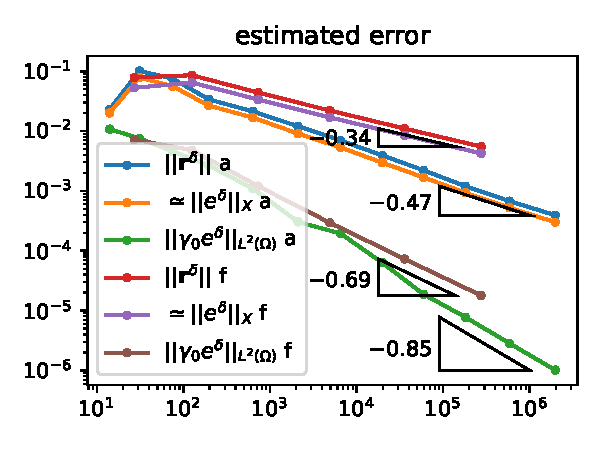
\includegraphics[width=0.5\linewidth]{smooth_adaptive_errors}
  \caption{Error progression of $e^\delta := u - u^{\underline{\delta}\delta}$ for the smooth problem as
  a function of $\dim X^\delta$ for adaptive and full grid refinement.\jw{excuse the terrible graph}}
  \label{fig:smooth}
\end{figure}

\subsection{First singular solution}
Selecting the L-shaped domain $\Omega := [-1,1]^2 \setminus [0,1]^2$ with data
$u_0 \equiv 0$ and $g(x,y) := \bbone_{{x^2 + y^2 \leq 1/4}}(x,y)$, the true
solution is unknown in closed form but known to be singular in the re-entrant
corner.\jw{is het wel singulier? of alleen minder regulier? hier wil ik een citatie of *iets* anders} Figure~\ref{fig:cylinder}
shows the error progression

\begin{itemize}
  \item Adaptive vs full vs sparse grid
  \item Misschien de spatial meshes voor wat verschillende $\lambda$, of sowieso
    tellen hoeveel $\lambda$'s er zijn in dit geval? lijkt veel op de numres van FK19
\end{itemize}
\begin{figure}
  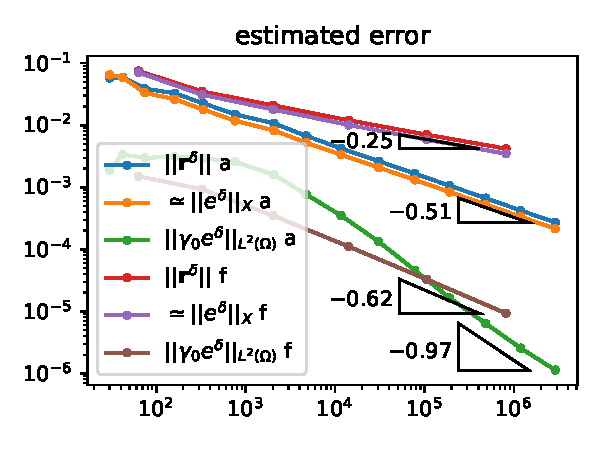
\includegraphics[width=0.5\linewidth]{cylinder_adaptive_errors}
  \caption{Error progression of $e^\delta := u - u^{\underline{\delta}\delta}$ for the cylinder problem as
  a function of $\dim X^\delta$ for adaptive and full grid refinement.\jw{excuse the terrible graph}}
  \label{fig:cylinder}
\end{figure}

\subsection{Second singular solution}
Selecting again the unit-square domain $\Omega := [0,1]^2$ with data $u_0 := \bbone$
and $g \equiv 0$, we see BLA.

\begin{itemize}
  \item Adaptive vs full vs sparse grid
  \item Memory en time graphs
\end{itemize}
\begin{figure}
  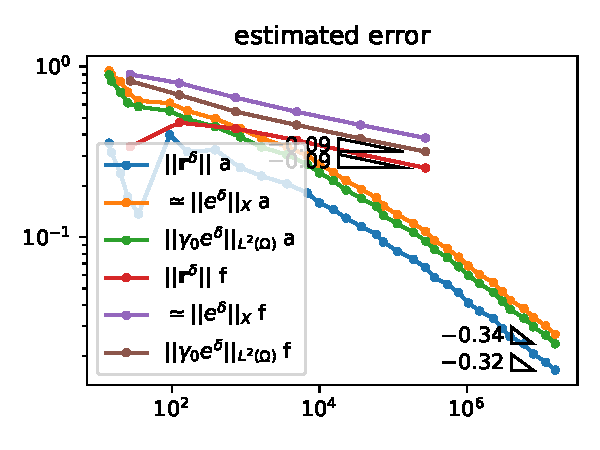
\includegraphics[width=0.5\linewidth]{singular_adaptive_errors}
  \caption{Error progression of $e^\delta := u - u^{\underline{\delta}\delta}$ for the singular problem as
  a function of $\dim X^\delta$ for adaptive and full grid refinement.\jw{excuse the terrible graph}}
  \label{fig:singular}
\end{figure}



\bibliography{library} 
\bibliographystyle{siam}

\end{document}
